% TEXINPUTS=.:$HOME/git/bvtex: latexmk  -pdf <main>.tex
\documentclass[xcolor=dvipsnames]{beamer}

\input{defaults}
\input{beamer/preamble}

\setbeamertemplate{navigation symbols}{}
% \setbeamertemplate{background}[grid][step=1cm]

\usepackage{siunitx}
\usepackage{xmpmulti}
\usepackage[export]{adjustbox}

\usepackage[outline]{contour}
\usepackage{tikz}
\usetikzlibrary{shapes.geometric, arrows}
\usetikzlibrary{positioning}

\definecolor{bvtitlecolor}{rgb}{0.98, 0.92, 0.84}
\definecolor{bvoutline}{rgb}{0.1, 0.1, 0.1}

\renewcommand{\bvtitleauthor}{Brett Viren\\\small for the BNL Wire Cell Group}
\renewcommand{\bvtit}{Wire Cell}
\renewcommand{\bvtitle}{\LARGE Wire Cell Event Reconstruction Software
for LArTPC Detectors}
\renewcommand{\bvevent}{BNL CSC Seminar 2015 Sep 29}
\renewcommand{\bvbeamerbackground}{}

% http://tex.stackexchange.com/a/23550
\makeatletter
\providecommand{\beamer@slideinframe}{0}%
\tikzset{highlight/.code={\ifnum#1=\beamer@slideinframe \tikzset{draw=red,text=red}\fi},highlight/.value required}
\makeatother

\setbeamertemplate{headline}{%
\leavevmode%
  \hbox{%
    \begin{beamercolorbox}[wd=\paperwidth,ht=2.5ex,dp=1.125ex]{palette quaternary}%
    \insertsectionnavigationhorizontal{\paperwidth}{}{\hskip0pt plus1filll}
    \end{beamercolorbox}%
  }
}
\begin{document}
\input{beamer/title.tex}
\input{beamer/toc.tex}

\lstset{%
  language=C++,
                basicstyle=\scriptsize\ttfamily,
                keywordstyle=\color{blue}\ttfamily,
                stringstyle=\color{red}\ttfamily,
                commentstyle=\color{gray}\ttfamily,
                morecomment=[l][\color{magenta}]{\#}
}

\section {Introduction}

\begin{frame}
  \frametitle{Who, What, Why}

  \begin{description}
  \item[who] \textbf{Wire Cell} development is centered in the
    \textbf{Electronic Detector Group}, of the \textbf{BNL Physics
      Department}.
  \item[what] Our focus is the experimental study of the properties of
    \textbf{neutrinos} and \textbf{muons}.
  \item[why] Our neutrino detectors are \textbf{Liquid Argon Time
      Proportion Chambers} (LArTPC), a technology \textbf{pioneered by
      BNL} since 1974.
  \end{description}
  Main Physics interests:
  \begin{itemize}
  \item Observe CP symmetry violation in neutrino interactions.
  \item Determination of neutrino mass ordering.
  \item Precision measurement of neutrino oscillation parameters.
  \item Observation of neutrino bursts from supernova explosions.
  \item Search for Proton decay and sterile neutrino.
  \end{itemize}
\end{frame}

\begin{frame}
  \frametitle{Why LArTPC}
  Measuring neutrino interactions require detectors that are:
  \begin{description}\footnotesize
  \item[big] active mass of \num{10} -- \SI{100}{\kilo\tonne}'s to
    mitigate tiny neutrino interaction cross sections.
  \item[efficient] capture of neutrino interactions
  \item[accurate] measure of energy, neutrino flavor and interaction type (ie, very good signal
    vs. background).
  \item[quiet] low background environment shielded against
    cosmic-$\mu$ and natural radioactivity, $\Rightarrow$ deep
    underground + active shielding.
  \end{description}

  Two main technologies:
  \begin{description}\footnotesize
  \item[Water Cherenkov] big++, efficient++, accurate+, quiet+\\
    simple understood technology modest S/B.
  \item[LArTPC] big+, eficient++, accurate++, quiet++, \\
    R\&D still improving, excellent future potential.
  \end{description}

  Many challenges still to overcome, but LArTPC's promises make it the
  chosen technology for future Neutrino experiments in the US.
\end{frame}

\begin{frame}
  \frametitle{LArTPC Experiments - Icarus}

  \begin{columns}
    \begin{column}{0.5\textwidth}
      \begin{itemize}
      \item Two \SI{300}{\tonne} modules in Gran Sasso tunnel, Italy.
      \item Took data from CERN neutrino beam.
      \item Moving to Fermilab as part of the \textbf{Short-Baseline
        Neutrino} Program.
      \end{itemize}
    \end{column}
    \begin{column}{0.5\textwidth}
      \includegraphics[width=0.8\textwidth]{icarus.png}
    \end{column}
  \end{columns}
\end{frame}

\begin{frame}
  \frametitle{LArTPC Experiments - MicroBooNE}

  \begin{columns}
    \begin{column}{0.5\textwidth}
      \begin{center}
        \includegraphics[width=0.9\textwidth]{run1148_ev1016.png}
      \end{center}

    \end{column}
    \begin{column}{0.5\textwidth}
      \begin{itemize}
      \item \SI{85}{\tonne} fiducial mass.
      \item 8256 channels
      \item 3 mm wire pitch.
      \item Investigate LSND-effect, look for sterile-$\nu$, measure $\nu$-Ar
        cross sections.
      \end{itemize}
    \end{column}
  \end{columns}

  \begin{center}
    Just started taking data at Fermilab!    
  \end{center}

  MicroBooNE is the initial test bed for Wire Cell reconstruction.

\end{frame}

\begin{frame}[fragile]
  \frametitle{LArTPC Experiments - 
\includegraphics[height=7mm,trim=4cm 9.2cm 4cm 9.3cm,clip,valign=c]{DUNElogo_colorHORIZONTAL.pdf}}
  \begin{center}
    ``International \textbf{mega-science} project''
  \end{center}

  Three stages of LArTPC detectors:
  \begin{enumerate}\footnotesize
  \item ``\textbf{35ton}'' prototype (at FNAL) commissioning now, running early 2016.
  \item Full-scale ``\textbf{protoDUNE}'' (at CERN) 2017 with $\pi, K, p$ beam tests.
  \item Full ``\textbf{DUNE}'' far detector underground in South Dakota $\sim$2025.
    \begin{itemize}
    \item \textbf{40 kt fiducial mass} in 4 modules.
    \item 5 mm wire pitch, \textbf{1.5M channels}.
    \end{itemize}
  \end{enumerate}
  Full DUNE: \textbf{underground + size} $\Rightarrow$ must design for: \textbf{wrapped
    induction wires} and \textbf{two sided anode planes}.\\
  $\rightarrow$ extra challenges to event reconstruction!

  \begin{center}
    \includegraphics[height=25mm]{LBNF_Graphic_021715-1024x340.png}
  \end{center}

\end{frame}

\begin{frame}
  \begin{center}
    Next: primer on how LArTPC works.
  \end{center}
\end{frame}

\begin{frame}[fragile]
  LArTPC = \textbf{L}iquid \textbf{Ar}gon \textbf{T}ime \textbf{P}roportional \textbf{C}hamber

  \begin{center}
      \transduration<0-16>{0}
      \multiinclude[<+->][format=png, graphics={height=0.7\textheight}]{signal}
  \end{center}

  \begin{minipage}[t][1cm]{1.0\textwidth}
    \only<1>{Charged particles traverse the detector at relativistic
      speeds and leave behind ionized Argon.}

    \only<2>{Ion and electron pairs drift off in opposite directions
      in the E-field applied between anode wires and cathode plane.}

    \only<3>{Here we watch the electrons drift.
      They drift with a speed of
      \SI{1.6}{\milli\meter\per\micro\second} toward the anode wire planes.}

    \only<4>{As they approach, they begin to induce signals on the
      nearby wires.}

    \only<5>{There are two planes of induction wires which see a
      bipolar signal as charge drifts by.}

    \only<6>{The final plane collects the drifting charge and thus sees a unipolar signal.}

    \only<7>{The exact signal response is complicated and depends on
      details of the electric field and detector construction.}

    \only<8>{Charge on each wire is digitized as a function of time.
      Typical digitization ``tick'' is
      \SI{0.5}{\micro\second}, wire spacing is \num{3} to \SI{5}{\milli\meter}.}

    \only<9>{Measuring the drifted charge requires a deconvolution of a
      response function and a noise filter with the raw wire signals.}

    \only<10>{As a batch of electrons drift, it diffuses out in both
      the longitudinal and transverse directions. LAr impurities cause
      attenuation.} 

    \only<11>{At the maximum drift distance allowed by the
      detector, diffusion can be as much as \SI{1}{\micro\second}
      longitudinally and \SI{2.5}{\milli\meter} transverse.} 

    
    \only<12>{Still drifting...} 
    
    \only<13>{Still drifting...
    It's a slow detector!}
    
    \only<14>{Still drifting...} 

    \only<15>{Each wire plane reads out one 2D view (wire pitch
      direction vs. time) of the drifting charge pattern.}
    
    \only<16>{Combining three 2D views can give a tomographic
      reconstruction of the particle trajectories and their energies.}
    
    \only<17>{Traditional methods work in 2D first, then combine
      assuming track-like hypothesis.
      OTOH, Wire Cell goes directly to 3D imaging.}

  \end{minipage}

\end{frame}

\begin{frame}
  \frametitle{Data Numerology}
  
  \vspace{-10mm}

  \begin{columns}
    \begin{column}{0.8\textwidth}
      LArTPC can produce prodigious quantities of data:
      \begin{itemize}
      \item $10^4$ -- $10^6$ channels
      \item 2MHz @ 12 bit FADC digitization
      \item each ``event'' spans several milliseconds
      \end{itemize}
    \end{column}
    \begin{column}{0.2\textwidth}
      \begin{center}
        \includegraphics[width=\textwidth,trim=13cm 0cm 0cm 0cm,clip]{signal-15.png}

        \scriptsize \SI{0.5}{\micro\second} waveform digitization.
      \end{center}
    \end{column}
  \end{columns}

  \vspace{-5mm}

  \footnotesize
  Two DAQ modes:
  \begin{description}
  \item[full-stream] read out entire waveform (\textbf{MicroBooNE})
    \begin{itemize}
    \item \textbf{30GB/s in 120 MB chunks}.
    \item DUNE would produce 3TB/s in 12 GB chunks.
    \end{itemize}
  \item[zero-supression] drop waveform chunks below a threshold (\textbf{DUNE})
    \begin{itemize}
    \item Threshold based on noise ($E_{equiv} <$\SI{0.5}{\mega\electronvolt})
    \item 2.5 MB/event $\rightarrow$ \textbf{100's TB/year}
    \item 50 PB/year if $^{39}$Ar decay backgrounds can not be
      rejected by DAQ.
    \end{itemize}
  \end{description}

\end{frame}


\section{Technique}

\begin{frame}[fragile]
  \frametitle{Wire Cell Reconstruction Method}
  \setbeamercovered{transparent}
  \begin{columns}
    \begin{column}{0.7\textwidth}
      Four main parts:
      \begin{enumerate}
      \item<2> Data Preparation
        \begin{itemize}        \scriptsize
        \item Construct wire and cell geometry.
        \item Read framed stream, form time slices
        \end{itemize}
      \item<3> Imaging of Activity
        \begin{itemize}        \scriptsize
        \item Identify 3D regions of space that likely contain
          activity consistent with wire signals.
        \end{itemize}
      \item<4> Pattern Recognition 
        \begin{itemize}         \scriptsize
        \item Cluster in space and time
        \item Categorize as track/shower
        \end{itemize}
      \item<5> Physics
        \begin{itemize}
        \item Determine particle ID and kinematics of tracks/showers.
        \end{itemize}
      \end{enumerate}
    \end{column}
    \begin{column}{0.3\textwidth}
      \begin{center}
        \vspace{-10mm}
        \resizebox{!}{\textheight}{
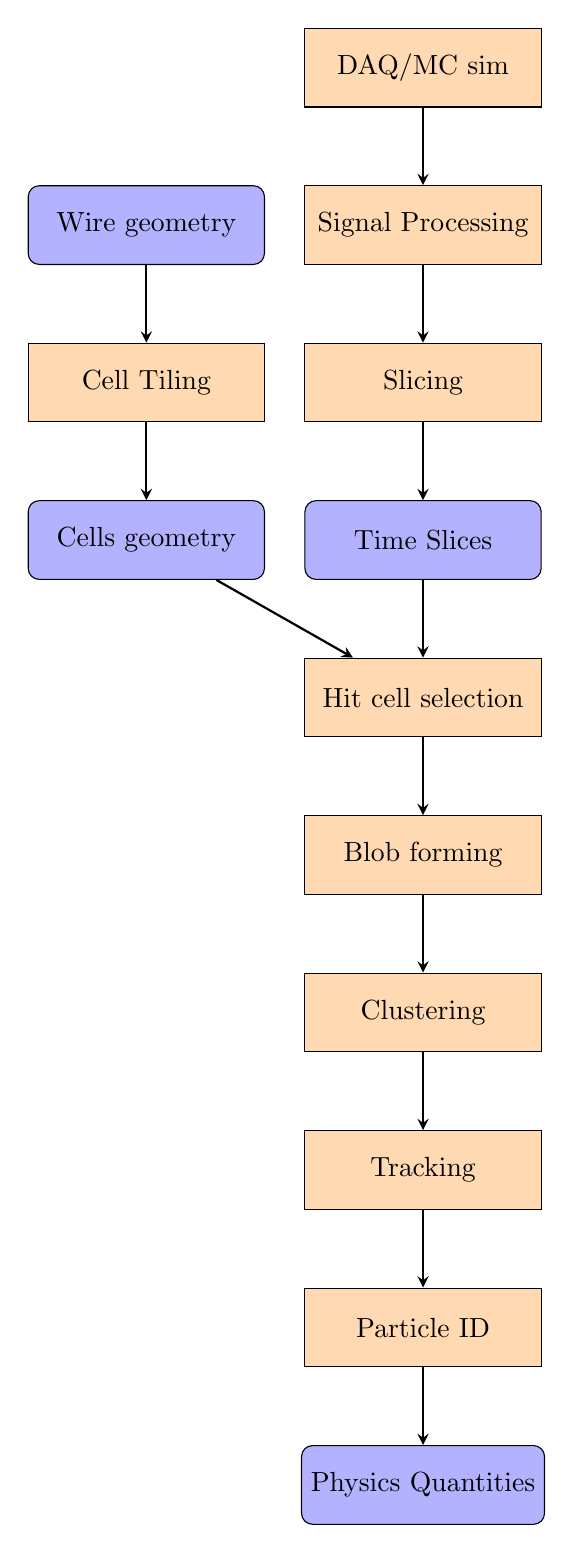
\begin{tikzpicture}[align=center, node distance=2cm]

\tikzstyle{dataobj} = [rectangle, rounded corners, minimum width=3cm, minimum height=1cm,text centered, draw=black, fill=blue!30]
\tikzstyle{process} = [rectangle, minimum width=3cm, minimum height=1cm, text centered, draw=black, fill=orange!30]
\tikzstyle{decision} = [diamond, minimum width=3cm, minimum height=1cm, text centered, draw=black, fill=green!30]
\tikzstyle{arrow} = [thick,->,>=stealth]

\node (daqmc) [process,highlight=2] {DAQ/MC sim};
\node (frames) [process,highlight=2, below of=daqmc] {Signal Processing};
\node (slicing) [process,highlight=2, below of=frames] {Slicing};
\node (slices) [dataobj, below of=slicing] {Time Slices};
\node (wires) [dataobj, left=0.5cm of frames] {Wire geometry};
\node (tiling) [process,highlight=2, left=0.5cm of slicing] {Cell Tiling};
\node (cells) [dataobj, left=0.5cm of slices] {Cells geometry};
\node (hitcells) [process,highlight=3, below of=slices] {Hit cell selection};
\node (blobbing) [process,highlight=3, below of=hitcells] {Blob forming};
\node (clustering) [process,highlight=4, below of=blobbing] {Clustering};
\node (tracking) [process,highlight=4, below of=clustering] {Tracking};
\node (pid) [process,highlight=5, below of=tracking] {Particle ID};
\node (physics) [dataobj, below of=pid] {Physics Quantities};

\draw [arrow] (wires) -- (tiling);
\draw [arrow] (tiling) -- (cells);
\draw [arrow] (cells) -- (hitcells);
\draw [arrow] (daqmc) -- (frames);
\draw [arrow] (frames) -- (slicing);
\draw [arrow] (slicing) -- (slices);
\draw [arrow] (slices) -- (hitcells);
\draw [arrow] (hitcells) -- (blobbing);
\draw [arrow] (blobbing) -- (clustering);
\draw [arrow] (clustering) -- (tracking);
\draw [arrow] (tracking) -- (pid);
\draw [arrow] (pid) -- (physics);
\end{tikzpicture}}
      \end{center}
    \end{column}
  \end{columns}

\end{frame}

\subsection{Data Preparation}

\begin{frame}
  \frametitle{Framing}
  
  \vspace{-2.0cm}
  \begin{center}
    \rotatebox{-90}{\includegraphics[width=6cm]{framing.pdf}}    
  \end{center}
  \vspace{-1.0cm}

  \scriptsize
  Raw data stream readout in blocks or \textbf{frames} of time.

  Typical digitizing: $\sim$\SI{4}{\milli\second}, \SI{2}{\mega\hertz}, 12 bit/sample.

  \begin{columns}
    \begin{column}{0.5\textwidth}
      \scriptsize
      \textbf{MicroBooNE:}
      \begin{itemize}
      \item \textbf{Very active at surface}: $\sim$20 cosmic-$\mu$ events/frame.
      \item Very ``few'' channels (8256).
      \item \textbf{full-stream} readout frames, big but manageable:
        \textbf{$\sim$100 MB/frame}.
      \end{itemize}

    \end{column}
    \begin{column}{0.5\textwidth}
      \scriptsize
      
      \textbf{DUNE:}
      \begin{itemize}
      \item \textbf{Deep underground}, quiet detector.
      \item Isolated $^{39}$Ar decays dominant bkg.
      \item \textbf{1.5M channels} could produce: \\
        4.5 TB/second \textbf{full-stream}!
      \item DUNE must \textbf{zero-suppress} signals.
      \item \textbf{$\sim$2.5 MB/frame} (25 GB if no ZS!)
      \item requires \textbf{clever DAQ!}
      \end{itemize}

    \end{column}
  \end{columns}
\end{frame}

\begin{frame}[fragile]
  \frametitle{Time Slicing}
  
  \begin{columns}
    \begin{column}{0.35\textwidth}
      \begin{center}
        \vspace{-.5cm}

        \includegraphics[width=\textwidth]{slice.pdf}

        \vspace{-2cm}

        \includegraphics[width=\textwidth,trim=0cm 10cm 0cm 0cm,clip]{slice-3D.pdf}

        \scriptsize True hits.
      \end{center}
    \end{column}
    \begin{column}{0.6\textwidth}

      \includegraphics[width=\textwidth]{wires-and-true-hits.png}

      \begin{itemize} \scriptsize
      \item One \textbf{time slice} of the frame.
      \item Slice width is chosen to match electronics shaping time: 4
        FADC ``ticks'' = \SI{2}{\micro\second}.
      \item Identify selection of ``hit'' wires in the slice.
        \begin{itemize} \scriptsize
        \item[$\rightarrow$] hit = FADC charge above some threshold.
        \end{itemize}
      \end{itemize}
    \end{column}
  \end{columns}

\end{frame}

\subsection{Imaging Of Activity}

\begin{frame}[fragile]
  \frametitle{Tiling}

  \begin{center}
    \includegraphics[width=0.7\textwidth,trim=8.6cm 9cm 8.6cm 9cm,clip]{test_boundcells.pdf}

    Zoom in on the wires and their associated cells.
  \end{center}



  \footnotesize
  \begin{itemize}
  \item Associate a 2D ``cell'' with small region near every
    triple-crossing of one wire from each plane.
  \item Cells completely tile the plane, no gaps, no overlaps.
  \item Cell shapes and sizes depend on wire plane pitches, angles and
    offsets.
  \end{itemize}

  \textbf{The heart of the Wire Cell concept:} if all three
  triple-crossing wires are ``hit'', the associated cell likely
  contains drifted charge.

\end{frame}

\begin{frame}
  \frametitle{Cell Ambiguity - Example Hit Pattern}

  \begin{columns}
    \begin{column}{0.5\textwidth}
      \includegraphics[width=\textwidth,trim=1cm 4cm 2cm 1cm,clip]{example-hit-cells.pdf}
    \end{column}
    \begin{column}{0.5\textwidth}
      Ambiguity arises due to spatial multiplexing.
      \begin{description}\scriptsize
      \item[Good] wire v3 measures no charge, all its cells must be unhit.
      \item[Bad] surrounding hits induce ``ghost'' at \textbf{c4}.
      \item[Ambiguous] multiple cells measured by same wire.
      \end{description}
      In some cases ambiguity can not be resolved at the cell level.
    \end{column}
  \end{columns}
\end{frame}

\begin{frame}[fragile]
  \frametitle{Some Formalism}
  Expected charge measured on \textbf{wires} ($\vec{w}$) can be calculated
  knowing charge in \textbf{cells} ($\vec{c}$):

  \[\vec{w} = \mathbf{G_{wc}}\vec{c}\]

  $\mathbf{G_{wc}}$ is the wire/cell \textit{adjacency matrix}, purely
  geometrical and perfectly known, function of detector design.
  
  \begin{columns}
    \begin{column}{0.45\textwidth}
      \vspace{-5mm}

      \flushright \includegraphics[width=0.8\textwidth,trim=1cm 11cm 2cm 2cm,clip]{example-hit-cells.pdf}

    \end{column}
    \begin{column}{0.10\textwidth}
      $\Leftrightarrow$
    \end{column}
    \begin{column}{0.45\textwidth}

  \resizebox{0.7\textwidth}{!}{
    $\left(
      \begin{array}[h]{c}
        0.0\\
        1.0\\
        2.0\\
        2.0\\
        0.0\\

        1.0\\
        1.0\\
        0.0\\
        2.0\\
        1.0\\

        1.0\\
        2.0\\
        2.0\\
      \end{array}
    \right)
    = \left(
      \begin{array}[h]{ccccccccc}
        1&0&0&0&0&0&0&0&0\\
        0&1&0&1&0&0&0&0&0\\
        0&0&1&0&1&0&1&0&0\\
        0&0&0&0&0&1&0&1&0\\
        0&0&0&0&0&0&0&0&1\\

        0&0&0&0&0&0&1&0&0\\
        0&0&0&1&0&0&0&1&0\\
        1&0&0&0&1&0&1&0&0\\
        0&1&0&0&0&1&0&0&0\\
        0&0&1&0&0&0&0&0&0\\
        
        1&0&0&1&0&0&1&0&0\\
        0&1&0&0&1&0&0&1&0\\
        0&0&1&0&0&1&0&0&1\\
      \end{array}
    \right)
    \left(
      \begin{array}[h]{c}
        0.0\\
        1.0\\
        1.0\\
        0.0\\
        0.0\\
        1.0\\
        1.0\\
        1.0\\
        0.0\\
      \end{array}
    \right)$}
      
    \end{column}
  \end{columns}


  Wish to solve inverse: $\vec{c} = \mathbf{G_{wc}}^{-1}\vec{w}$.
  However, $N_{cells} \approx N_{wires}^2$ \\
  $\Rightarrow$ as $N_{cells}$ grows, more unknowns ($\vec{c}$) than knowns ($\vec{w}$)!
\end{frame}

\begin{frame}
  \frametitle{Form Blobs}
  \vspace{-10mm}
  \begin{columns}
    \begin{column}{0.5\textwidth}
      Goal: \textbf{reduce matrix size} and \textbf{remove ambiguity}.
    \end{column}
    \begin{column}{0.5\textwidth}
      \includegraphics[width=0.8\textwidth]{wires-and-true-hits.png}          
    \end{column}
  \end{columns}
      
  \begin{enumerate}
  \item Select all cells with all three wires ``hit''.
  \item Partition into spatially contiguous subsets: ``\textbf{blobs}''.
  \end{enumerate}
  Equation to solve is now:
  \[\vec{w_b} = \mathbf{G_{wb}} \vec{b}\]

  \begin{description}
  \item[$\vec{c} \to \vec{b}$] vector of charge in each blob.
  \item[$\mathbf{G_{wc}} \to \mathbf{G_{wb}}$] the wire-blob adjacency matrix for the slice.
  \item[$\vec{w} \to \vec{w_b}$] vector of charge on all wires associated with blob.
  \end{description}

\end{frame}

% maybe remove this slide...
\begin{frame}
  \frametitle{Another wrinkle: charge uncertainty}

  Measures of the drifting charge by a wire has uncertainty.
  \begin{itemize}
  \item Noise from electronics and thermal fluctuations.
  \item Statistical uncertainty due to digitization.
  \item Systematic uncertainties from detector response deconvolution.
  \item Can be correlated across wires.
  \end{itemize}
  Compare measured wire charge ($\vec{w}_{meas}$) with expected
  ($\vec{w}_{exp}$) and form a $\chi^2$ with $\mathrm{V}$ a
  covariance uncertainty matrix.
  
  \[\chi^2 = (\vec{w}_{meas}-\vec{w}_{exp})^\intercal\mathrm{V}^{-1} (\vec{w}_{meas}-\vec{w}_{exp})\]

  ``It can be shown'' that minimizing this $\chi^2$ is equivalent to
  inverting $\mathbf{G_{wc}}$ (or $\mathbf{G_{wb}}$) matrix equation.

\end{frame}

\begin{frame}[fragile]
  \frametitle{The Payoff: imaged \SI{3}{\giga\electronvolt} $\nu_e$ interaction}
  
  \begin{columns}
    \begin{column}{0.5\textwidth}
      \begin{center}
        \includegraphics[width=\textwidth,trim=0cm 10cm 0cm 0cm,clip]{payoff-true.png}

        True energy depositions.
      \end{center}
    \end{column}
    \begin{column}{0.5\textwidth}
      \begin{center}
        \includegraphics[width=\textwidth,trim=0cm 10cm 0cm 0cm,clip]{payoff-reco.png}

        Wire Cell imaging.
      \end{center}
    \end{column}
  \end{columns}
  \footnotesize
  \begin{itemize}
  \item Excellent imaging of major track features as well as isolated
    activity.
    \begin{itemize}\scriptsize
    \item[$\rightarrow$] a static 2D view doesn't do it justice!  \href{http://www.phy.bnl.gov/wire-cell/bee/set/6/event/0/}{See it for yourself.}
    \end{itemize}
  \item Remaining ambiguity seen as wide blue patches.
    \begin{itemize}\scriptsize
    \item[$\rightarrow$] inherent in LArTPC technology, Wire Cell makes it evident.
    \end{itemize}
  \end{itemize}
\end{frame}


\subsection{Pattern Recognition}

\begin{frame}
  \frametitle{Clustering, Tracking and Categorization}
  Post-imaging, current approach:
  \begin{enumerate}
  \item \textbf{cluster} together blobs contiguous in space and time
    (slice).
  \item \textbf{track} a line through a cluster.
  \item \textbf{categorize} success/failure of line to account for the
    cluster's charge distribution.
  \end{enumerate}
  Some categories:
  \begin{description}
  \item[track] cluster is well fit by the track
  \item[short] cluster appears to be a ``short track'' (eg, $\delta$-ray)
  \item[shower] cluster appears to be a EM/hadronic shower
  \item[undefined] no well-suited categorization.
  \end{description}

  \begin{itemize}
  \item Active area of Wire Cell development.
  \item May benefit from collaboration with machine learning experts. 
  \end{itemize}

\end{frame}

\subsection{Physics}
\begin{frame}
  \frametitle{Physics-level Reconstruction}

  This development is just beginning.
  
  It will:
  \begin{itemize}
  \item associate clusters with a particle trajectory
  \item determine particle type
  \item determine momentum, range, dE/dx and other kinematics.
  \end{itemize}

\end{frame}


\section{Software Design}

\begin{frame}
  \tableofcontents[currentsection,hideothersubsections]
\end{frame}

\subsection{Software Overview}

\begin{frame}
  \frametitle{Wire Cell Software Ecosystem}

  Wire Cell breaks up into three main parts:

  \begin{description}
  \item[visualization] the ``Bee'' web application (Chao Zhang)
  \item[prototype] reconstruction algorithms, initial proof of
    principle (Xin Qian)
  \item[toolkit] ``production'' toolkit for LArTPC reconstruction (bv)
  \end{description}

\end{frame}

\subsection{Bee Display}

\begin{frame}
  \frametitle{Bee Features}

  Bee is a 3D interactive visualization system:
  \begin{itemize}
  \item Displays results of different reconstruction algorithms.
  \item Shows ``true'' particle trajectories from simulation.
  \item Very good for developers to debug and compare different
    methods and for users to gain Physics/LArTPC intuition.
  \item Implemented as \textbf{JavaScript/WebGL} front-end and
    \textbf{Django} back-end.
  \item Works on popular desktop and mobile browsers.
  \item Requires hardware WebGL support.
  \item JSON data file format, easy to implement schema.
  \item Supports drag-and-drop
    \href{http://bnlif.github.io/wire-cell-docs/viz/uploads/}{user
      file uploads}.
  \item New features almost daily (\textbf{Chao Zhang}!)
  \end{itemize}
\end{frame}

\begin{frame}[fragile]
  \frametitle{Bee: Select and upload event sets}
  \begin{center}
    \includegraphics[height=0.8\textheight]{bee-event-sets-page.png}

    \vspace{-3cm}
    \flushright \footnotesize Simple JSON format\\
    \includegraphics[width=3cm]{json-data.png}
  \end{center}
\end{frame}

\begin{frame}
  \frametitle{Interactive 3D visualization}
  \begin{center}
    \includegraphics[height=0.7\textheight]{bee-full-gui.png}    
  \end{center}
  \begin{center}
    Try it yourself! \url{http://www.phy.bnl.gov/wire-cell/bee/}
  \end{center}
\end{frame}


\subsection{Prototype}

\begin{frame}
  \frametitle{Wire Cell Working Prototype}
  \footnotesize

  \begin{itemize}
  \item \textbf{Very successful proof of principle!}
  \item Currently \textbf{leads the state of the art} in LArTPC
    reconstruction techniques.
  \item Amazingly fast development (\textbf{Xin Qian}!)
    \begin{itemize}\scriptsize
    \item[$\rightarrow$] Work started only $\sim$5 months ago!
    \end{itemize}
  \end{itemize}

  \begin{center}
    \includegraphics[height=0.5\textheight,trim=0cm 0cm 0cm 2cm,clip]{xin-shower.png}

    \scriptsize
    Colors indicate identified tracks and showers.
  \end{center}

\end{frame}

\begin{frame}
  \frametitle{Compromises to Remedy}

  Some compromises were accepted for the rapid prototype and now need
  ``back-filling''.  Need to remedy:

  \begin{itemize}
  \item No support for long-term, multi-developer contributions.
  \item Many monolithic, single-threaded applications.
  \item Hard-coded ``magic'' numbers.
  \item Rigid code structure and hard-coded workflows.
  \item Exchange files are only integration with external frameworks.
  \item Need comprehensive CPU/memory optimization campaign.
  \item Some tests but better coverage/granularity needed.
  \item Intimate dependency on the large
    ROOT\footnote{\url{https://root.cern.ch/}} toolkit.
  \end{itemize}

  Decision: rewrite rather than refactor $\longrightarrow$
  
\end{frame}

\subsection{Toolkit}

\begin{frame}
  \frametitle{Wire Cell Toolkit}
  \begin{columns}
    \begin{column}{0.65\paperwidth}
    \end{column}
    \begin{column}{0.35\paperwidth}
      \vspace{-20mm}
      \includegraphics[width=\textwidth]{deps.pdf}      
    \end{column}
  \end{columns}

  \vspace{-15mm}

  High level overview:
  \begin{itemize}
  \item Includes \textbf{packaging and build} system.
  \item Comprehensive \textbf{API} via abstract base classes.
  \item Mindful of \textbf{dependencies}, external and internal.
  \item Built-in wire and cell \textbf{geometry descriptions} or load from file.
  \item Includes simple \textbf{LArTPC detector simulation}.
  \item Refactored implementations of core \textbf{prototype algorithms}.
  \item Abstracted \textbf{execution model}, step towards parallelism.
  \item Support for native and foreign \textbf{file I/O}.
  \item Follow ``toolkit'' software paradigm.
  \end{itemize}

\end{frame}

\begin{frame}[fragile]
  \frametitle{Source Repositories and Build}

  \begin{itemize}
  \item Code in GitHub \href{https://github.com/WireCell/}{WireCell} organization.
  \item Code aggregation with \textbf{git submodule}.
  \item A simple, customized \href{https://waf.io/}{waf}-based build.\footnote{\texttt{wcb} = \texttt{waf} + extra Waf tools for Boost, ROOT, Eigen and Wire Cell packaging}
  

  \end{itemize}

  \begin{lstlisting}{langauge=shell}
$ git clone git@github.com:WireCell/wire-cell.git
$ cd wire-cell/
$ git submodule init
$ git submodule update
$ ./wcb --prefix=/path/to/install configure build install
  \end{lstlisting}
%$

  Builds, tests and installs:
  \begin{itemize}
  \item toolkit shared libraries + header files,
  \item main applications,
  \item many unit tests,
  \item \href{http://www.phy.bnl.gov/wire-cell/doxy/html/}{Doxygen reference} and \href{http://wirecell.github.io/wire-cell-docs/}{MkDocs user documentation}.
  \end{itemize}


\end{frame}

\begin{frame}[fragile]
  \frametitle{Wire Cell Interfaces}

  The \href{https://github.com/WireCell/wire-cell-iface}{\texttt{wire-cell-iface}} package:

  \begin{itemize}
  \item API composed of abstract base classes covering:
    \begin{itemize}
    \item \textbf{Data model} (wires, cells, frames, slices, tracks, ...)
    \item \textbf{Active components} (blob maker, matrix solver, clustering, ...)
    \end{itemize}
  \item Use of C++ \verb|shared_ptr<>| for (mostly) \textbf{worry-free memory management}.
  \item Dynamic instance lookup via \texttt{NamedFactory} pattern
    allows for a \textbf{plugin architecture}.
  \item Initial support for \textbf{user configuration} system based on Boost
    property trees.
  \item Initial support exists for an \textbf{abstract execution model}.
  \end{itemize}
\end{frame}

\begin{frame}

  \frametitle{Wire Cell Simulation}

  \begin{columns}
    \begin{column}{0.75\textwidth}
      \begin{itemize}\footnotesize
      \item Provided by the \href{https://github.com/WireCell/wire-cell-gen}{\texttt{wire-cell-gen}} package.
      \item Simple implementation of the 4 ``D''s of LArTPC:\\
        \textbf{deposit, drift, diffuse, digitize}.
      \item Granular, user may tak as little or as much as needed.
        \begin{itemize}\scriptsize
        \item[$\rightarrow$] Parts can be replaced by external
          simulation, \\or bypassed entirely with real DAQ data.
        \item[$\rightarrow$] External integration via file I/O or API calls.
        \end{itemize}
      \item Provides reference implementation to guide external frameworks integrator/developers.
      \item Useful for quickly generating data to feed unit tests.
      \end{itemize}
    \end{column}
    \begin{column}{0.25\textwidth}
      \vspace{-10mm}
      \includegraphics[width=\textwidth]{sim-flow.pdf}
    \end{column}
  \end{columns}
\end{frame}

\begin{frame}[fragile]
  \frametitle{Wire Cell Execution Model}

  \begin{columns}
    \begin{column}{0.7\textwidth}
      \footnotesize 
      The toolkit supports \textbf{data flow programming} paradigm
      \begin{itemize}
        \item Directly influenced by \href{http://www0.bnl.gov/events/details.php?q=8932}{CSC Seminar on VisTrails, March 2013}!
        \item Data flows through a graph made from:
          \begin{description}
          \item[vertices] computational units / algorithms
          \item[edges] data queues of a given type
          \end{description}
        \item Vertex has well defined input/output data types.
        \item Edges can be thread-safe queues.
        \item Streamed data, minimizing unneeded buffering.
        \item Graph-level ``programming'' to define workflows.
        \item Graph execution machinery swapable: uniproc, multiproc, or
          distributed (MPI) parallel.
        \item Encourages isolated, targeted development and testing of each
          compute vertex.
        \item Feedback loops to implement iterative workflows.
        \item Instrument graph to collect performance data.
        \end{itemize}
      \end{column}
      \begin{column}{0.3\textwidth}

        \vspace{-10mm}

        \includegraphics[width=\textwidth]{dataflow.pdf}
      \end{column}
    \end{columns}
\end{frame}

\begin{frame}
  \frametitle{Abstract execution model}

  \scriptsize Want to swap execution model while leaving ``real'' algorithm code untouched!

\footnotesize
  
  \begin{columns}
    \begin{column}{0.6\textwidth}
      Each graph vertex made from three layers.  From outside to in:
      \begin{enumerate}
      \item Execution model layer implementing data flow control
        \begin{itemize}\scriptsize
        \item sync'ed load-and-flush, async, multi-processing, message-passing, ...
        \end{itemize}
      \item Adapter between actual algorithm and execution model ``client''.
      \item Algorithm implementation and interface unrestricted except ``no shared
        globals'' 
      \end{enumerate}
    \end{column}
    \begin{column}{0.4\textwidth}
      \includegraphics[width=1.1\textwidth]{concentric.pdf}      
    \end{column}
  \end{columns}

\end{frame}

\section{Future Plans}

\begin{frame}
  \tableofcontents[currentsection,hideothersubsections]
\end{frame}

\begin{frame}\frametitle{Future Plans}
  \begin{center}
    ...in which I frequently beg for help : )
  \end{center}
\end{frame}

\subsection{Algorithm Development}

\begin{frame}
  \frametitle{Pattern Recognition}
  It is turning out to be ``hard''.
  \footnotesize
  \begin{itemize}
  \item Many challenges are \textbf{inherent to the LArTPC technology}.  
    \begin{itemize}\scriptsize
    \item[$\rightarrow$] Wire Cell has just allowed us to reach them.
    \end{itemize}
  \item Current implementation is largely \textbf{heuristic based}
    \begin{itemize}\scriptsize
    \item many ``cross-algorithm assumptions''
    \item \textbf{large solution space} with \textbf{many corner cases}.
    \item human Physicists find good, \textbf{per-event/ad-hoc solutions}.
    \item[$\rightarrow$] but how to teach them to the computer?
    \end{itemize}
  \item[$\rightarrow$] Our attempt: Bee 2.0 (next slide) 
  \end{itemize}
  
  We feel we may be entering to the area of ``real'' computer science
  problems like machine learning.

  \vspace{2mm}

  And we are not experts. 

  \vspace{2mm}

  \textbf{Help Wanted!}

\end{frame}

\subsection{Bee 2.0}


\begin{frame}
  \frametitle{Bee 2.0: Human-directed Automated Reconstruction}
  Interim Solution: inject human judgment to guide Wire Cell reconstruction.
  \begin{enumerate}
  \item Bee will let humans \textbf{interactively control reconstruction}.
    \begin{itemize}
    \item ``Join cluster X to cluster Y''
    \item ``Remove blob AAA from cluster Z''
    \end{itemize}
  \item Convert human commands into operational objects.
  \item Send to back end, execute inside a Wire Cell service.
  \item Send results back to user.
  \item Record everything in a database to mine for potential Wire
    Cell improvements.
  \end{enumerate}
  Think: ``\textbf{Physics-PhotoShop}'' + ``\textbf{Google Analytics}''.

\end{frame}

\begin{frame}
  \frametitle{Bee 2.0: Architecture}
  Plans include:
  \begin{itemize}
  \item Move Bee from \href{http://threejs.org/}{\texttt{three.js}} to a new JS/WebGL framework to support interactive controls (eg ``picking'').
  \item Develop a web-friendly \textbf{batch workflow system} (probably based on Celery) to run Wire Cell promptly.
  \item Develop a \textbf{database} system to capture ``analytics'' and coordinate the system (likely to use MongoDB).
  \item Develop the Django \textbf{middleware} to tie this all together.
  \item Provision the \textbf{hardware} to support all this (at BNL).
  \end{itemize}

  Early ideas but conceptually a \texttt{rather big} system.

  \textbf{Help wanted!}

\end{frame}

\subsection{Parallel Wire Cell}

\begin{frame}
  \frametitle{Wire Cell Production Processing}

  A 1-2 punch for today's computing:
  \begin{itemize}\footnotesize
  \item[$\rightarrow$] Need high thoughput to keep up with detector data rates.
  \item[$\rightarrow$] Need high performance due to CPU-heavy algorithms.
  \end{itemize}

  \footnotesize

  \begin{columns}
    \begin{column}{0.70\textwidth}
      Data volumes:
      \begin{description}
      \item[MicroBooNE] $\sim$630 TB/year (compressed)
      \item[protoDUNE] $\mathcal{O}$(1PB) total, (ZS, uncomp.)
      \item[DUNE 40kt] $\mathcal{O}$(PB)/year (ZS, uncomp.)
      \end{description}
      \begin{itemize}
      \item Okay, it's not quite ATLAS-levels 
        \begin{itemize}\scriptsize
        \item Run 1 produced $\sim$3PB/year raw.
        \end{itemize}
      \item \textbf{Wire Cell needs raw wire data}
        \begin{itemize}\scriptsize
        \item No Level-X triggers to save you.
        \item MicroBooNE: offline sees full-stream, no-ZS.
        \item Surface protoDUNE: $\sim$60 cosmic-$\mu$s per readout.
        \item Underground DUNE: all detector activity is sacred.
        \end{itemize}
      \item Current speed: \textbf{30 minutes -- 1day / event!}
        \begin{itemize}\scriptsize
        \item Optimization expected, etc, etc, but:  \textbf{gulp!}
        \end{itemize}
      \end{itemize}
    \end{column}
    \begin{column}{0.30\textwidth}
      \begin{center}
        \includegraphics[width=\textwidth,trim=5cm 9cm 3cm 6cm,clip]{frank-abuse.pdf}

        \scriptsize (with apologies to \href{https://www.bnl.gov/events/details.php?q=11000}{Frank Wuerthwein})
      \end{center}
    \end{column}
  \end{columns}

\end{frame}

\begin{frame}
  \frametitle{Taking Wire Cell Parallel}

  Plans are focused on implementing parallel execution models:

  \begin{enumerate}\footnotesize
  \item \href{https://github.com/erenon/pipeline}{Boost.Pipeline} nice
    and simple threaded data flow package.  Easy to start with but not
    yet officially part of BOOST (longevity concerns?).
  \item \href{https://www.threadingbuildingblocks.org/}{Intel TBB} a
    common and well supported library with a fantastic looking ``flow
    graph designer'' tool.  Some effort needed to learn/adopt.
  \item MPI/ZeroMQ or other ways to run Wire Cell as multiple-node
    distributed process (maybe on \textbf{HPC}).  Big learning curve
    for us.
  \item Investigate potential for \textbf{GPU/Phi} hardware
    acceleration.  \\ Even bigger learning curve!
  \end{enumerate}

  This level of parallelism is \textbf{new ground for us}\footnote{This is a subject of a pending Computing LDRD proposal.}.

  \textbf{Help wanted!}
\end{frame}


\section{}

\begin{frame}
  \frametitle{Summary}
  \footnotesize
  \begin{itemize}
  \item The \textbf{Wire Cell working prototype LArTPC reconstruction} method and software has been developed.
    \begin{itemize}
    \item already producing some of the world's best results,
    \item technical and performance improvements still needed.
    \end{itemize}
  \item The \textbf{Bee interactive 3D event visualization}
    application developed, critical for understanding LArTPC and
    developing Wire Cell.  Plans to evolve to ``human-directed
    automated reconstruction''.
  \item The \textbf{Wire Cell Toolkit} for LArTPC reconstruction
    partly complete and will be the basis for long term development
    including investigations into parallel processing.
  \item To be successful we are going into \textbf{new waters} (for
    us) of parallel processing, hardware acceleration, computing
    science and mathematics.
    \begin{itemize}
    \item[$\rightarrow$] \textbf{Expert input, help and collaboration is most welcome!}
    \end{itemize}
  \end{itemize}
\end{frame}

\begin{frame}
  \frametitle{Wire Cell on the web}

  \begin{itemize}
  \item home page: \\ \url{http://www.phy.bnl.gov/wire-cell/}
  \item Bee entry: \\ \url{http://www.phy.bnl.gov/wire-cell/bee/}
  \item prototype user manual: \\ \url{http://bnlif.github.io/wire-cell-docs/}
  \item toolkit user manual: \\ \url{http://wirecell.github.io/wire-cell-docs/}
  \item toolkit reference: \\ \url{http://www.phy.bnl.gov/wire-cell/doxy/html/}
  \item prototype repositories: \\ \url{https://github.com/BNLIF}
  \item toolkit repositories: \\ \url{https://github.com/WireCell}
  \end{itemize}
\end{frame}

\end{document}


%%% Local Variables:
%%% mode: latex
%%% TeX-master: t
%%% End:
